\chapter{Background}
When designing the new Autograder front-end, it was necessary to develop other parts of the system for emulating dummy-data for the project. One of the most conventional ways of doing this is to create a database that stores the dummy-data, and have a server serve the front-end with that data. The system works in many ways as the fully functional Autograder, with predefined protocols for communications so that the new front-end can be implemented and deployed with a relatively small amount of effort. Making these protocols require us to both think about the current needs and future needs. Even though the system is currently up and running, many new ways of communicating with the new front-end is planned and will be implemented in the new system. It is however, no small task to create these sub-systems. We will go though some of the technologies we are using in this chapter.


\section{Planning phase}
Planning the new Autograder took many iterations of design and layout. The programming phase is simplified if all the layout has been planned ahead. All actions, tasks and functions of the site must be mapped out. New functionality must also be incorporated into the new design. The next section will show how the new layout has been planned and designed.

The more traditional way of designing a website is to start with wireframes. Wireframes are basic sketches or mockups of the design. The most basic forms does not include colors or advanced shapes. Simple boxes and rectangles are used to get a feel for how the page will look and function. The process starts with a revisit of the old Autograder front-end. All functions and tasks of all users must be mapped out. This includes functions such as approval of labs, signing in, making groups etc. The tasks are mapped using a technique called \emph{User Stories}. User stories are verbal guides to map all functionality. Stories come in the form \emph{"As a <role>, I want to <goal> so that <benefit>"}. Here are some of the user stories that Autograder uses;

\begin{itemize*}
\item As a student i want to create new group, so that other students can join for group assignment.
\item As an admin I want to list all current students so that I can manage permissions (admin,teacher,student).
\item As a teacher I want to archive / delete course, so that I can see only relevant and active courses.
\end{itemize*}


User stories help plan the whole system. The order of which functions are implemented can be managed from the start. In Autograder's case, functions like listing labs for the teacher will be a high priority user story. Functions like changing the group names can wait until a later point in development. Using a spreadsheet such as Excel to write the user stories is a productive way of planning the page. Each role of the page, i.e students, teachers and admins can be placed in different columns. User stories for each column is then written in rows. Trello was used, because of the "card"-design that the page has. Moving the cards is made easy through a drag-and-drop interface. This makes the job of managing the user stories much more simple, and it can also be used throughout the development as a TODO list.


\begin{figure}[h!]
    \centering
    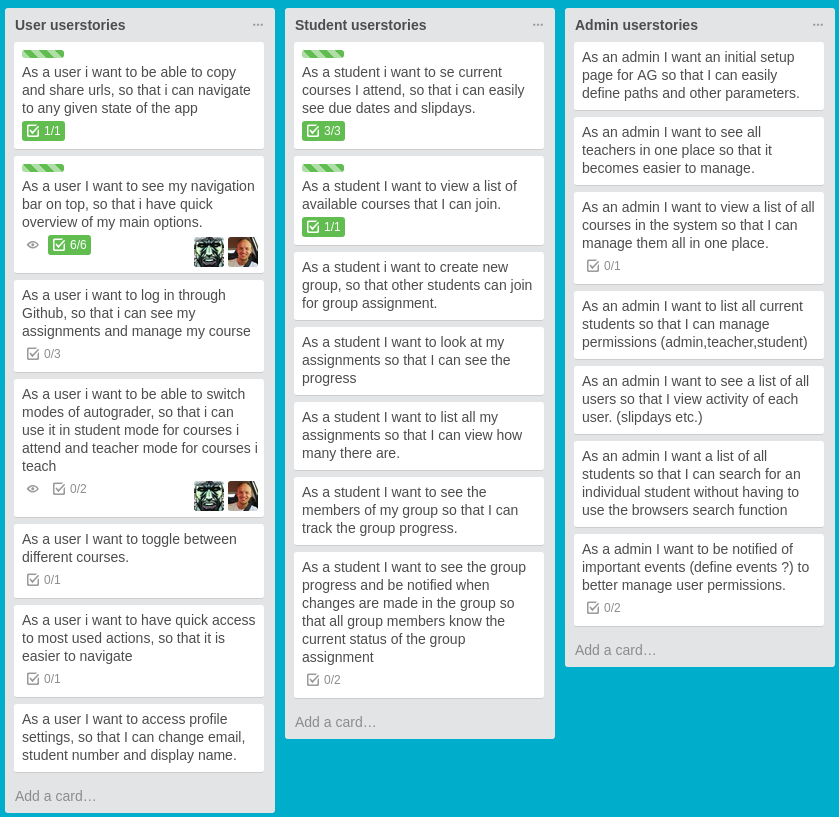
\includegraphics[width=0.8\textwidth]{./graphs/trello.png}
    \caption{Autograder's Trello page. Comprised of user stories, it was used as a TODO-list in the development process. Note: this is meant as an illustrative figure.}
    \label{fig:View of the trello page we used}
\end{figure}

The above image shows how we used Trello as a tool in the development process. The user stories are written down as cards. The cards can then be moved around.
\\User stories can also be used to make Wireframes. As said, students, teachers and admins each have their own user stories. The stories are usually drawn into wireframes with the client present. In our case, we talked to Professor Hein Meling at UiS, which acted as the client for the new Autograder front-end. Using the feedback the was given, the design evolved through many versions. Pages such as the results view \worry{ref til figur/wireframe} went though many iterations before landing on the final layout.



\section{Front-end}
Making the new Autograder requires us to make a website to show and control all the systems that work in the back. Pages for showing grades, students, groups, teahers and admins have to be made. This includes pages for managing the system and so on. Traditional webdesign takes a lot of time, where the process normally involves creating a design, coding the content and then styling the page. HTML (HyperText Markup Language) and CSS (Cascading Style Sheets) is the most used way of showing content and styling it, however, this process takes a lot of time, and frankly, is in most cases the boring part of the job.
\\Making the new Autograder requires a solid framework for HTML and CSS that removed the need to hard-code every DOM-element (Document object model), and make future expanding to make the application mobile friendly easier. It was decided early on to use \textit{Twitter Bootstrap} [ref to about page]. The framework is in it's third iteration (soon 4th with Bootstrap 4.0 Alpha being shipped early 2016). Bootstrap removes the need to make all the elements of the page, by using predefined components placed on the page. The framework comes with build in styling, so the job of the designer (or rather lack of designers) is made easier. Compared to vanilla coding in HTML and CSS, the framework can remove countless of hours of coding, and the results look clean and functional. \\As with the JavaScript and data binding, we use React. React is an open source JavaScript library designed and maintained by Facebook \worry{ref here}. The framework provides a view for data rendered as HTML, and maintains a state that can change depending on the data that comes from the server. This removes a lot of overhead programming that the developers usually have to think about. If the data in the server changes, the change is reflected on the frontpage in realtime. Say for example that the users rights are changed from Student to Teacher. The frontend will have to reflect that change, and show data relevant for a teacher. With React, this change can be made without having to update the page manually. The document object model, DOM for short, is always updated. Updating of elements and data on the page is one of Reacts strongest sides, therefore, it is a very good library for Autograder frontend. \\The choice between ReactJS and AngularJS (the other big JavaScript-library in the industry) is really based on preference. The component based pipeline that React offers is very appealing when the website will recycle a lot of the same elements. The new frontend can be compared to a single-page-application, where the different pages are loaded in without refreshing the page. Normally this requires a lot of loading and unloading of elements, and ReactJS already have this build in to the framework. \\ReactJS uses Virtual DOM to run its Tree Diff algorythm and figures out what parts of the DOM should be rendered, this enables quick re-rendering of only relevant for the change components.

\begin{figure}[h]
\centering
\scalebox{0.5}{\scalefont{1.8}{% Graphic for TeX using PGF
% Title: /home/tomgli/workspace/github.com/bachopp/thesis/files/chapters/background/graphs/reactdiffdiagramthin.dia
% Creator: Dia v0.97.3
% CreationDate: Sat Apr 23 13:55:59 2016
% For: tomgli
% \usepackage{tikz}
% The following commands are not supported in PSTricks at present
% We define them conditionally, so when they are implemented,
% this pgf file will use them.
\ifx\du\undefined
  \newlength{\du}
\fi
\setlength{\du}{15\unitlength}
\begin{tikzpicture}
\pgftransformxscale{1.000000}
\pgftransformyscale{-1.000000}
\definecolor{dialinecolor}{rgb}{0.000000, 0.000000, 0.000000}
\pgfsetstrokecolor{dialinecolor}
\definecolor{dialinecolor}{rgb}{1.000000, 1.000000, 1.000000}
\pgfsetfillcolor{dialinecolor}
\definecolor{dialinecolor}{rgb}{1.000000, 1.000000, 1.000000}
\pgfsetfillcolor{dialinecolor}
\pgfpathellipse{\pgfpoint{34.909398\du}{57.597439\du}}{\pgfpoint{0.922067\du}{0\du}}{\pgfpoint{0\du}{0.874328\du}}
\pgfusepath{fill}
\pgfsetlinewidth{0.100000\du}
\pgfsetdash{}{0pt}
\pgfsetdash{}{0pt}
\pgfsetmiterjoin
\definecolor{dialinecolor}{rgb}{0.000000, 0.000000, 0.000000}
\pgfsetstrokecolor{dialinecolor}
\pgfpathellipse{\pgfpoint{34.909398\du}{57.597439\du}}{\pgfpoint{0.922067\du}{0\du}}{\pgfpoint{0\du}{0.874328\du}}
\pgfusepath{stroke}
% setfont left to latex
\definecolor{dialinecolor}{rgb}{0.000000, 0.000000, 0.000000}
\pgfsetstrokecolor{dialinecolor}
\node at (34.909398\du,57.792439\du){};
\definecolor{dialinecolor}{rgb}{1.000000, 1.000000, 1.000000}
\pgfsetfillcolor{dialinecolor}
\pgfpathellipse{\pgfpoint{34.925608\du}{60.858968\du}}{\pgfpoint{0.922067\du}{0\du}}{\pgfpoint{0\du}{0.874328\du}}
\pgfusepath{fill}
\pgfsetlinewidth{0.100000\du}
\pgfsetdash{}{0pt}
\pgfsetdash{}{0pt}
\pgfsetmiterjoin
\definecolor{dialinecolor}{rgb}{0.000000, 0.000000, 0.000000}
\pgfsetstrokecolor{dialinecolor}
\pgfpathellipse{\pgfpoint{34.925608\du}{60.858968\du}}{\pgfpoint{0.922067\du}{0\du}}{\pgfpoint{0\du}{0.874328\du}}
\pgfusepath{stroke}
% setfont left to latex
\definecolor{dialinecolor}{rgb}{0.000000, 0.000000, 0.000000}
\pgfsetstrokecolor{dialinecolor}
\node at (34.925608\du,61.053968\du){};
\definecolor{dialinecolor}{rgb}{1.000000, 1.000000, 1.000000}
\pgfsetfillcolor{dialinecolor}
\pgfpathellipse{\pgfpoint{39.675251\du}{57.895710\du}}{\pgfpoint{0.922067\du}{0\du}}{\pgfpoint{0\du}{0.874328\du}}
\pgfusepath{fill}
\pgfsetlinewidth{0.100000\du}
\pgfsetdash{}{0pt}
\pgfsetdash{}{0pt}
\pgfsetmiterjoin
\definecolor{dialinecolor}{rgb}{0.000000, 0.000000, 0.000000}
\pgfsetstrokecolor{dialinecolor}
\pgfpathellipse{\pgfpoint{39.675251\du}{57.895710\du}}{\pgfpoint{0.922067\du}{0\du}}{\pgfpoint{0\du}{0.874328\du}}
\pgfusepath{stroke}
% setfont left to latex
\definecolor{dialinecolor}{rgb}{0.000000, 0.000000, 0.000000}
\pgfsetstrokecolor{dialinecolor}
\node at (39.675251\du,58.090710\du){};
\definecolor{dialinecolor}{rgb}{1.000000, 0.509804, 0.509804}
\pgfsetfillcolor{dialinecolor}
\pgfpathellipse{\pgfpoint{38.686418\du}{62.486491\du}}{\pgfpoint{0.922067\du}{0\du}}{\pgfpoint{0\du}{0.874328\du}}
\pgfusepath{fill}
\pgfsetlinewidth{0.100000\du}
\pgfsetdash{}{0pt}
\pgfsetdash{}{0pt}
\pgfsetmiterjoin
\definecolor{dialinecolor}{rgb}{0.000000, 0.000000, 0.000000}
\pgfsetstrokecolor{dialinecolor}
\pgfpathellipse{\pgfpoint{38.686418\du}{62.486491\du}}{\pgfpoint{0.922067\du}{0\du}}{\pgfpoint{0\du}{0.874328\du}}
\pgfusepath{stroke}
% setfont left to latex
\definecolor{dialinecolor}{rgb}{0.000000, 0.000000, 0.000000}
\pgfsetstrokecolor{dialinecolor}
\node at (38.686418\du,62.681491\du){};
\definecolor{dialinecolor}{rgb}{0.898039, 0.898039, 0.898039}
\pgfsetfillcolor{dialinecolor}
\fill (48.025035\du,46.743799\du)--(48.025035\du,48.643799\du)--(51.299533\du,48.643799\du)--(51.299533\du,46.743799\du)--cycle;
\pgfsetlinewidth{0.100000\du}
\pgfsetdash{}{0pt}
\pgfsetdash{}{0pt}
\pgfsetmiterjoin
\definecolor{dialinecolor}{rgb}{0.549020, 0.549020, 0.549020}
\pgfsetstrokecolor{dialinecolor}
\draw (48.025035\du,46.743799\du)--(48.025035\du,48.643799\du)--(51.299533\du,48.643799\du)--(51.299533\du,46.743799\du)--cycle;
% setfont left to latex
\definecolor{dialinecolor}{rgb}{0.000000, 0.000000, 0.000000}
\pgfsetstrokecolor{dialinecolor}
\node at (49.662284\du,47.888799\du){};
\definecolor{dialinecolor}{rgb}{0.898039, 0.898039, 0.898039}
\pgfsetfillcolor{dialinecolor}
\fill (46.210841\du,49.629967\du)--(46.210841\du,51.529967\du)--(49.485338\du,51.529967\du)--(49.485338\du,49.629967\du)--cycle;
\pgfsetlinewidth{0.100000\du}
\pgfsetdash{}{0pt}
\pgfsetdash{}{0pt}
\pgfsetmiterjoin
\definecolor{dialinecolor}{rgb}{0.549020, 0.549020, 0.549020}
\pgfsetstrokecolor{dialinecolor}
\draw (46.210841\du,49.629967\du)--(46.210841\du,51.529967\du)--(49.485338\du,51.529967\du)--(49.485338\du,49.629967\du)--cycle;
% setfont left to latex
\definecolor{dialinecolor}{rgb}{0.000000, 0.000000, 0.000000}
\pgfsetstrokecolor{dialinecolor}
\node at (47.848090\du,50.774967\du){};
\definecolor{dialinecolor}{rgb}{0.898039, 0.898039, 0.898039}
\pgfsetfillcolor{dialinecolor}
\fill (50.571434\du,49.649420\du)--(50.571434\du,51.549420\du)--(53.845932\du,51.549420\du)--(53.845932\du,49.649420\du)--cycle;
\pgfsetlinewidth{0.100000\du}
\pgfsetdash{}{0pt}
\pgfsetdash{}{0pt}
\pgfsetmiterjoin
\definecolor{dialinecolor}{rgb}{0.549020, 0.549020, 0.549020}
\pgfsetstrokecolor{dialinecolor}
\draw (50.571434\du,49.649420\du)--(50.571434\du,51.549420\du)--(53.845932\du,51.549420\du)--(53.845932\du,49.649420\du)--cycle;
% setfont left to latex
\definecolor{dialinecolor}{rgb}{0.000000, 0.000000, 0.000000}
\pgfsetstrokecolor{dialinecolor}
\node at (52.208683\du,50.794420\du){};
\definecolor{dialinecolor}{rgb}{0.898039, 0.898039, 0.898039}
\pgfsetfillcolor{dialinecolor}
\fill (44.038649\du,52.385733\du)--(44.038649\du,54.285733\du)--(47.313147\du,54.285733\du)--(47.313147\du,52.385733\du)--cycle;
\pgfsetlinewidth{0.100000\du}
\pgfsetdash{}{0pt}
\pgfsetdash{}{0pt}
\pgfsetmiterjoin
\definecolor{dialinecolor}{rgb}{0.549020, 0.549020, 0.549020}
\pgfsetstrokecolor{dialinecolor}
\draw (44.038649\du,52.385733\du)--(44.038649\du,54.285733\du)--(47.313147\du,54.285733\du)--(47.313147\du,52.385733\du)--cycle;
% setfont left to latex
\definecolor{dialinecolor}{rgb}{0.000000, 0.000000, 0.000000}
\pgfsetstrokecolor{dialinecolor}
\node at (45.675898\du,53.530733\du){};
\definecolor{dialinecolor}{rgb}{0.898039, 0.898039, 0.898039}
\pgfsetfillcolor{dialinecolor}
\fill (48.399243\du,52.405185\du)--(48.399243\du,54.305185\du)--(51.673740\du,54.305185\du)--(51.673740\du,52.405185\du)--cycle;
\pgfsetlinewidth{0.100000\du}
\pgfsetdash{}{0pt}
\pgfsetdash{}{0pt}
\pgfsetmiterjoin
\definecolor{dialinecolor}{rgb}{0.549020, 0.549020, 0.549020}
\pgfsetstrokecolor{dialinecolor}
\draw (48.399243\du,52.405185\du)--(48.399243\du,54.305185\du)--(51.673740\du,54.305185\du)--(51.673740\du,52.405185\du)--cycle;
% setfont left to latex
\definecolor{dialinecolor}{rgb}{0.000000, 0.000000, 0.000000}
\pgfsetstrokecolor{dialinecolor}
\node at (50.036492\du,53.550185\du){};
\definecolor{dialinecolor}{rgb}{0.898039, 0.898039, 0.898039}
\pgfsetfillcolor{dialinecolor}
\fill (48.512715\du,55.368444\du)--(48.512715\du,57.268444\du)--(51.787213\du,57.268444\du)--(51.787213\du,55.368444\du)--cycle;
\pgfsetlinewidth{0.100000\du}
\pgfsetdash{}{0pt}
\pgfsetdash{}{0pt}
\pgfsetmiterjoin
\definecolor{dialinecolor}{rgb}{0.549020, 0.549020, 0.549020}
\pgfsetstrokecolor{dialinecolor}
\draw (48.512715\du,55.368444\du)--(48.512715\du,57.268444\du)--(51.787213\du,57.268444\du)--(51.787213\du,55.368444\du)--cycle;
% setfont left to latex
\definecolor{dialinecolor}{rgb}{0.000000, 0.000000, 0.000000}
\pgfsetstrokecolor{dialinecolor}
\node at (50.149964\du,56.513444\du){};
\definecolor{dialinecolor}{rgb}{1.000000, 1.000000, 1.000000}
\pgfsetfillcolor{dialinecolor}
\pgfpathellipse{\pgfpoint{31.922753\du}{56.062026\du}}{\pgfpoint{0.922067\du}{0\du}}{\pgfpoint{0\du}{0.874328\du}}
\pgfusepath{fill}
\pgfsetlinewidth{0.100000\du}
\pgfsetdash{}{0pt}
\pgfsetdash{}{0pt}
\pgfsetmiterjoin
\definecolor{dialinecolor}{rgb}{0.000000, 0.000000, 0.000000}
\pgfsetstrokecolor{dialinecolor}
\pgfpathellipse{\pgfpoint{31.922753\du}{56.062026\du}}{\pgfpoint{0.922067\du}{0\du}}{\pgfpoint{0\du}{0.874328\du}}
\pgfusepath{stroke}
% setfont left to latex
\definecolor{dialinecolor}{rgb}{0.000000, 0.000000, 0.000000}
\pgfsetstrokecolor{dialinecolor}
\node at (31.922753\du,56.257026\du){};
\definecolor{dialinecolor}{rgb}{0.898039, 0.898039, 0.898039}
\pgfsetfillcolor{dialinecolor}
\fill (47.984149\du,61.262534\du)--(47.984149\du,63.162534\du)--(51.258647\du,63.162534\du)--(51.258647\du,61.262534\du)--cycle;
\pgfsetlinewidth{0.100000\du}
\pgfsetdash{}{0pt}
\pgfsetdash{}{0pt}
\pgfsetmiterjoin
\definecolor{dialinecolor}{rgb}{0.549020, 0.549020, 0.549020}
\pgfsetstrokecolor{dialinecolor}
\draw (47.984149\du,61.262534\du)--(47.984149\du,63.162534\du)--(51.258647\du,63.162534\du)--(51.258647\du,61.262534\du)--cycle;
% setfont left to latex
\definecolor{dialinecolor}{rgb}{0.000000, 0.000000, 0.000000}
\pgfsetstrokecolor{dialinecolor}
\node at (49.621398\du,62.407534\du){};
\definecolor{dialinecolor}{rgb}{0.898039, 0.898039, 0.898039}
\pgfsetfillcolor{dialinecolor}
\fill (46.169955\du,64.148703\du)--(46.169955\du,66.048703\du)--(49.444453\du,66.048703\du)--(49.444453\du,64.148703\du)--cycle;
\pgfsetlinewidth{0.100000\du}
\pgfsetdash{}{0pt}
\pgfsetdash{}{0pt}
\pgfsetmiterjoin
\definecolor{dialinecolor}{rgb}{0.549020, 0.549020, 0.549020}
\pgfsetstrokecolor{dialinecolor}
\draw (46.169955\du,64.148703\du)--(46.169955\du,66.048703\du)--(49.444453\du,66.048703\du)--(49.444453\du,64.148703\du)--cycle;
% setfont left to latex
\definecolor{dialinecolor}{rgb}{0.000000, 0.000000, 0.000000}
\pgfsetstrokecolor{dialinecolor}
\node at (47.807204\du,65.293703\du){};
\definecolor{dialinecolor}{rgb}{0.898039, 0.898039, 0.898039}
\pgfsetfillcolor{dialinecolor}
\fill (50.530549\du,64.168155\du)--(50.530549\du,66.068155\du)--(53.805046\du,66.068155\du)--(53.805046\du,64.168155\du)--cycle;
\pgfsetlinewidth{0.100000\du}
\pgfsetdash{}{0pt}
\pgfsetdash{}{0pt}
\pgfsetmiterjoin
\definecolor{dialinecolor}{rgb}{0.549020, 0.549020, 0.549020}
\pgfsetstrokecolor{dialinecolor}
\draw (50.530549\du,64.168155\du)--(50.530549\du,66.068155\du)--(53.805046\du,66.068155\du)--(53.805046\du,64.168155\du)--cycle;
% setfont left to latex
\definecolor{dialinecolor}{rgb}{0.000000, 0.000000, 0.000000}
\pgfsetstrokecolor{dialinecolor}
\node at (52.167798\du,65.313155\du){};
\definecolor{dialinecolor}{rgb}{1.000000, 0.509804, 0.509804}
\pgfsetfillcolor{dialinecolor}
\fill (43.997764\du,66.904468\du)--(43.997764\du,68.804468\du)--(47.272261\du,68.804468\du)--(47.272261\du,66.904468\du)--cycle;
\pgfsetlinewidth{0.100000\du}
\pgfsetdash{}{0pt}
\pgfsetdash{}{0pt}
\pgfsetmiterjoin
\definecolor{dialinecolor}{rgb}{0.549020, 0.549020, 0.549020}
\pgfsetstrokecolor{dialinecolor}
\draw (43.997764\du,66.904468\du)--(43.997764\du,68.804468\du)--(47.272261\du,68.804468\du)--(47.272261\du,66.904468\du)--cycle;
% setfont left to latex
\definecolor{dialinecolor}{rgb}{0.000000, 0.000000, 0.000000}
\pgfsetstrokecolor{dialinecolor}
\node at (45.635013\du,68.049468\du){};
\definecolor{dialinecolor}{rgb}{0.898039, 0.898039, 0.898039}
\pgfsetfillcolor{dialinecolor}
\fill (48.358357\du,66.923920\du)--(48.358357\du,68.823920\du)--(51.632855\du,68.823920\du)--(51.632855\du,66.923920\du)--cycle;
\pgfsetlinewidth{0.100000\du}
\pgfsetdash{}{0pt}
\pgfsetdash{}{0pt}
\pgfsetmiterjoin
\definecolor{dialinecolor}{rgb}{0.549020, 0.549020, 0.549020}
\pgfsetstrokecolor{dialinecolor}
\draw (48.358357\du,66.923920\du)--(48.358357\du,68.823920\du)--(51.632855\du,68.823920\du)--(51.632855\du,66.923920\du)--cycle;
% setfont left to latex
\definecolor{dialinecolor}{rgb}{0.000000, 0.000000, 0.000000}
\pgfsetstrokecolor{dialinecolor}
\node at (49.995606\du,68.068920\du){};
\definecolor{dialinecolor}{rgb}{0.898039, 0.898039, 0.898039}
\pgfsetfillcolor{dialinecolor}
\fill (48.471830\du,69.887179\du)--(48.471830\du,71.787179\du)--(51.746328\du,71.787179\du)--(51.746328\du,69.887179\du)--cycle;
\pgfsetlinewidth{0.100000\du}
\pgfsetdash{}{0pt}
\pgfsetdash{}{0pt}
\pgfsetmiterjoin
\definecolor{dialinecolor}{rgb}{0.549020, 0.549020, 0.549020}
\pgfsetstrokecolor{dialinecolor}
\draw (48.471830\du,69.887179\du)--(48.471830\du,71.787179\du)--(51.746328\du,71.787179\du)--(51.746328\du,69.887179\du)--cycle;
% setfont left to latex
\definecolor{dialinecolor}{rgb}{0.000000, 0.000000, 0.000000}
\pgfsetstrokecolor{dialinecolor}
\node at (50.109079\du,71.032179\du){};
\definecolor{dialinecolor}{rgb}{1.000000, 1.000000, 1.000000}
\pgfsetfillcolor{dialinecolor}
\fill (67.651782\du,54.752294\du)--(67.651782\du,56.652294\du)--(70.926279\du,56.652294\du)--(70.926279\du,54.752294\du)--cycle;
\pgfsetlinewidth{0.100000\du}
\pgfsetdash{}{0pt}
\pgfsetdash{}{0pt}
\pgfsetmiterjoin
\definecolor{dialinecolor}{rgb}{0.000000, 0.000000, 0.000000}
\pgfsetstrokecolor{dialinecolor}
\draw (67.651782\du,54.752294\du)--(67.651782\du,56.652294\du)--(70.926279\du,56.652294\du)--(70.926279\du,54.752294\du)--cycle;
% setfont left to latex
\definecolor{dialinecolor}{rgb}{0.000000, 0.000000, 0.000000}
\pgfsetstrokecolor{dialinecolor}
\node at (69.289030\du,55.897294\du){};
\definecolor{dialinecolor}{rgb}{1.000000, 1.000000, 1.000000}
\pgfsetfillcolor{dialinecolor}
\fill (65.837587\du,57.638463\du)--(65.837587\du,59.538463\du)--(69.112085\du,59.538463\du)--(69.112085\du,57.638463\du)--cycle;
\pgfsetlinewidth{0.100000\du}
\pgfsetdash{}{0pt}
\pgfsetdash{}{0pt}
\pgfsetmiterjoin
\definecolor{dialinecolor}{rgb}{0.000000, 0.000000, 0.000000}
\pgfsetstrokecolor{dialinecolor}
\draw (65.837587\du,57.638463\du)--(65.837587\du,59.538463\du)--(69.112085\du,59.538463\du)--(69.112085\du,57.638463\du)--cycle;
% setfont left to latex
\definecolor{dialinecolor}{rgb}{0.000000, 0.000000, 0.000000}
\pgfsetstrokecolor{dialinecolor}
\node at (67.474836\du,58.783463\du){};
\definecolor{dialinecolor}{rgb}{1.000000, 1.000000, 1.000000}
\pgfsetfillcolor{dialinecolor}
\fill (70.198181\du,57.657915\du)--(70.198181\du,59.557915\du)--(73.472679\du,59.557915\du)--(73.472679\du,57.657915\du)--cycle;
\pgfsetlinewidth{0.100000\du}
\pgfsetdash{}{0pt}
\pgfsetdash{}{0pt}
\pgfsetmiterjoin
\definecolor{dialinecolor}{rgb}{0.000000, 0.000000, 0.000000}
\pgfsetstrokecolor{dialinecolor}
\draw (70.198181\du,57.657915\du)--(70.198181\du,59.557915\du)--(73.472679\du,59.557915\du)--(73.472679\du,57.657915\du)--cycle;
% setfont left to latex
\definecolor{dialinecolor}{rgb}{0.000000, 0.000000, 0.000000}
\pgfsetstrokecolor{dialinecolor}
\node at (71.835430\du,58.802915\du){};
\definecolor{dialinecolor}{rgb}{1.000000, 0.509804, 0.509804}
\pgfsetfillcolor{dialinecolor}
\fill (63.665396\du,60.394228\du)--(63.665396\du,62.294228\du)--(66.939894\du,62.294228\du)--(66.939894\du,60.394228\du)--cycle;
\pgfsetlinewidth{0.100000\du}
\pgfsetdash{}{0pt}
\pgfsetdash{}{0pt}
\pgfsetmiterjoin
\definecolor{dialinecolor}{rgb}{0.000000, 0.000000, 0.000000}
\pgfsetstrokecolor{dialinecolor}
\draw (63.665396\du,60.394228\du)--(63.665396\du,62.294228\du)--(66.939894\du,62.294228\du)--(66.939894\du,60.394228\du)--cycle;
% setfont left to latex
\definecolor{dialinecolor}{rgb}{0.000000, 0.000000, 0.000000}
\pgfsetstrokecolor{dialinecolor}
\node at (65.302645\du,61.539228\du){};
\definecolor{dialinecolor}{rgb}{1.000000, 1.000000, 1.000000}
\pgfsetfillcolor{dialinecolor}
\fill (68.025989\du,60.413680\du)--(68.025989\du,62.313680\du)--(71.300487\du,62.313680\du)--(71.300487\du,60.413680\du)--cycle;
\pgfsetlinewidth{0.100000\du}
\pgfsetdash{}{0pt}
\pgfsetdash{}{0pt}
\pgfsetmiterjoin
\definecolor{dialinecolor}{rgb}{0.000000, 0.000000, 0.000000}
\pgfsetstrokecolor{dialinecolor}
\draw (68.025989\du,60.413680\du)--(68.025989\du,62.313680\du)--(71.300487\du,62.313680\du)--(71.300487\du,60.413680\du)--cycle;
% setfont left to latex
\definecolor{dialinecolor}{rgb}{0.000000, 0.000000, 0.000000}
\pgfsetstrokecolor{dialinecolor}
\node at (69.663238\du,61.558680\du){};
\definecolor{dialinecolor}{rgb}{1.000000, 1.000000, 1.000000}
\pgfsetfillcolor{dialinecolor}
\fill (68.139462\du,63.376939\du)--(68.139462\du,65.276939\du)--(71.413960\du,65.276939\du)--(71.413960\du,63.376939\du)--cycle;
\pgfsetlinewidth{0.100000\du}
\pgfsetdash{}{0pt}
\pgfsetdash{}{0pt}
\pgfsetmiterjoin
\definecolor{dialinecolor}{rgb}{0.000000, 0.000000, 0.000000}
\pgfsetstrokecolor{dialinecolor}
\draw (68.139462\du,63.376939\du)--(68.139462\du,65.276939\du)--(71.413960\du,65.276939\du)--(71.413960\du,63.376939\du)--cycle;
% setfont left to latex
\definecolor{dialinecolor}{rgb}{0.000000, 0.000000, 0.000000}
\pgfsetstrokecolor{dialinecolor}
\node at (69.776711\du,64.521939\du){};
\pgfsetlinewidth{0.100000\du}
\pgfsetdash{}{0pt}
\pgfsetdash{}{0pt}
\pgfsetmiterjoin
\definecolor{dialinecolor}{rgb}{0.549020, 0.549020, 0.549020}
\pgfsetstrokecolor{dialinecolor}
\pgfpathellipse{\pgfpoint{49.127059\du}{51.603158\du}}{\pgfpoint{6.946203\du}{0\du}}{\pgfpoint{0\du}{6.480362\du}}
\pgfusepath{stroke}
% setfont left to latex
\definecolor{dialinecolor}{rgb}{0.000000, 0.000000, 0.000000}
\pgfsetstrokecolor{dialinecolor}
\node at (49.127059\du,51.798158\du){};
\pgfsetlinewidth{0.100000\du}
\pgfsetdash{}{0pt}
\pgfsetdash{}{0pt}
\pgfsetbuttcap
{
\definecolor{dialinecolor}{rgb}{0.549020, 0.549020, 0.549020}
\pgfsetfillcolor{dialinecolor}
% was here!!!
\definecolor{dialinecolor}{rgb}{0.549020, 0.549020, 0.549020}
\pgfsetstrokecolor{dialinecolor}
\draw (49.034225\du,48.692966\du)--(48.476148\du,49.580801\du);
}
\pgfsetlinewidth{0.100000\du}
\pgfsetdash{}{0pt}
\pgfsetdash{}{0pt}
\pgfsetbuttcap
{
\definecolor{dialinecolor}{rgb}{0.549020, 0.549020, 0.549020}
\pgfsetfillcolor{dialinecolor}
% was here!!!
\definecolor{dialinecolor}{rgb}{0.549020, 0.549020, 0.549020}
\pgfsetstrokecolor{dialinecolor}
\draw (50.538230\du,48.693315\du)--(51.332737\du,49.599903\du);
}
\pgfsetlinewidth{0.100000\du}
\pgfsetdash{}{0pt}
\pgfsetdash{}{0pt}
\pgfsetbuttcap
{
\definecolor{dialinecolor}{rgb}{0.549020, 0.549020, 0.549020}
\pgfsetfillcolor{dialinecolor}
% was here!!!
\definecolor{dialinecolor}{rgb}{0.549020, 0.549020, 0.549020}
\pgfsetstrokecolor{dialinecolor}
\draw (47.059769\du,51.580076\du)--(46.464219\du,52.335624\du);
}
\pgfsetlinewidth{0.100000\du}
\pgfsetdash{}{0pt}
\pgfsetdash{}{0pt}
\pgfsetbuttcap
{
\definecolor{dialinecolor}{rgb}{0.549020, 0.549020, 0.549020}
\pgfsetfillcolor{dialinecolor}
% was here!!!
\definecolor{dialinecolor}{rgb}{0.549020, 0.549020, 0.549020}
\pgfsetstrokecolor{dialinecolor}
\draw (48.635615\du,51.578666\du)--(49.248966\du,52.356486\du);
}
\pgfsetlinewidth{0.100000\du}
\pgfsetdash{}{0pt}
\pgfsetdash{}{0pt}
\pgfsetbuttcap
{
\definecolor{dialinecolor}{rgb}{0.549020, 0.549020, 0.549020}
\pgfsetfillcolor{dialinecolor}
% was here!!!
\definecolor{dialinecolor}{rgb}{0.549020, 0.549020, 0.549020}
\pgfsetstrokecolor{dialinecolor}
\draw (50.074791\du,54.355357\du)--(50.111664\du,55.318272\du);
}
\pgfsetlinewidth{0.100000\du}
\pgfsetdash{}{0pt}
\pgfsetdash{}{0pt}
\pgfsetbuttcap
{
\definecolor{dialinecolor}{rgb}{0.549020, 0.549020, 0.549020}
\pgfsetfillcolor{dialinecolor}
% was here!!!
\definecolor{dialinecolor}{rgb}{0.549020, 0.549020, 0.549020}
\pgfsetstrokecolor{dialinecolor}
\draw (48.993340\du,63.211701\du)--(48.435263\du,64.099536\du);
}
\pgfsetlinewidth{0.100000\du}
\pgfsetdash{}{0pt}
\pgfsetdash{}{0pt}
\pgfsetbuttcap
{
\definecolor{dialinecolor}{rgb}{0.549020, 0.549020, 0.549020}
\pgfsetfillcolor{dialinecolor}
% was here!!!
\definecolor{dialinecolor}{rgb}{0.549020, 0.549020, 0.549020}
\pgfsetstrokecolor{dialinecolor}
\draw (50.497345\du,63.212051\du)--(51.291851\du,64.118638\du);
}
\pgfsetlinewidth{0.100000\du}
\pgfsetdash{}{0pt}
\pgfsetdash{}{0pt}
\pgfsetbuttcap
{
\definecolor{dialinecolor}{rgb}{0.549020, 0.549020, 0.549020}
\pgfsetfillcolor{dialinecolor}
% was here!!!
\definecolor{dialinecolor}{rgb}{0.549020, 0.549020, 0.549020}
\pgfsetstrokecolor{dialinecolor}
\draw (47.018883\du,66.098811\du)--(46.423334\du,66.854359\du);
}
\pgfsetlinewidth{0.100000\du}
\pgfsetdash{}{0pt}
\pgfsetdash{}{0pt}
\pgfsetbuttcap
{
\definecolor{dialinecolor}{rgb}{0.549020, 0.549020, 0.549020}
\pgfsetfillcolor{dialinecolor}
% was here!!!
\definecolor{dialinecolor}{rgb}{0.549020, 0.549020, 0.549020}
\pgfsetstrokecolor{dialinecolor}
\draw (48.594730\du,66.097402\du)--(49.208081\du,66.875221\du);
}
\pgfsetlinewidth{0.100000\du}
\pgfsetdash{}{0pt}
\pgfsetdash{}{0pt}
\pgfsetbuttcap
{
\definecolor{dialinecolor}{rgb}{0.549020, 0.549020, 0.549020}
\pgfsetfillcolor{dialinecolor}
% was here!!!
\definecolor{dialinecolor}{rgb}{0.549020, 0.549020, 0.549020}
\pgfsetstrokecolor{dialinecolor}
\draw (50.033906\du,68.874092\du)--(50.070779\du,69.837007\du);
}
\pgfsetlinewidth{0.100000\du}
\pgfsetdash{}{0pt}
\pgfsetdash{}{0pt}
\pgfsetbuttcap
{
\definecolor{dialinecolor}{rgb}{0.000000, 0.000000, 0.000000}
\pgfsetfillcolor{dialinecolor}
% was here!!!
\definecolor{dialinecolor}{rgb}{0.000000, 0.000000, 0.000000}
\pgfsetstrokecolor{dialinecolor}
\draw (68.660972\du,56.701461\du)--(68.102895\du,57.589296\du);
}
\pgfsetlinewidth{0.100000\du}
\pgfsetdash{}{0pt}
\pgfsetdash{}{0pt}
\pgfsetbuttcap
{
\definecolor{dialinecolor}{rgb}{0.000000, 0.000000, 0.000000}
\pgfsetfillcolor{dialinecolor}
% was here!!!
\definecolor{dialinecolor}{rgb}{0.000000, 0.000000, 0.000000}
\pgfsetstrokecolor{dialinecolor}
\draw (70.164977\du,56.701811\du)--(70.959483\du,57.608398\du);
}
\pgfsetlinewidth{0.100000\du}
\pgfsetdash{}{0pt}
\pgfsetdash{}{0pt}
\pgfsetbuttcap
{
\definecolor{dialinecolor}{rgb}{0.000000, 0.000000, 0.000000}
\pgfsetfillcolor{dialinecolor}
% was here!!!
\definecolor{dialinecolor}{rgb}{0.000000, 0.000000, 0.000000}
\pgfsetstrokecolor{dialinecolor}
\draw (66.686515\du,59.588571\du)--(66.090966\du,60.344119\du);
}
\pgfsetlinewidth{0.100000\du}
\pgfsetdash{}{0pt}
\pgfsetdash{}{0pt}
\pgfsetbuttcap
{
\definecolor{dialinecolor}{rgb}{0.000000, 0.000000, 0.000000}
\pgfsetfillcolor{dialinecolor}
% was here!!!
\definecolor{dialinecolor}{rgb}{0.000000, 0.000000, 0.000000}
\pgfsetstrokecolor{dialinecolor}
\draw (68.262362\du,59.587162\du)--(68.875713\du,60.364981\du);
}
\pgfsetlinewidth{0.100000\du}
\pgfsetdash{}{0pt}
\pgfsetdash{}{0pt}
\pgfsetbuttcap
{
\definecolor{dialinecolor}{rgb}{0.000000, 0.000000, 0.000000}
\pgfsetfillcolor{dialinecolor}
% was here!!!
\definecolor{dialinecolor}{rgb}{0.000000, 0.000000, 0.000000}
\pgfsetstrokecolor{dialinecolor}
\draw (69.701538\du,62.363852\du)--(69.738411\du,63.326767\du);
}
\definecolor{dialinecolor}{rgb}{1.000000, 0.509804, 0.509804}
\pgfsetfillcolor{dialinecolor}
\fill (56.489531\du,58.272316\du)--(56.489531\du,60.172316\du)--(59.764029\du,60.172316\du)--(59.764029\du,58.272316\du)--cycle;
\pgfsetlinewidth{0.100000\du}
\pgfsetdash{}{0pt}
\pgfsetdash{}{0pt}
\pgfsetmiterjoin
\definecolor{dialinecolor}{rgb}{0.000000, 0.000000, 0.000000}
\pgfsetstrokecolor{dialinecolor}
\draw (56.489531\du,58.272316\du)--(56.489531\du,60.172316\du)--(59.764029\du,60.172316\du)--(59.764029\du,58.272316\du)--cycle;
% setfont left to latex
\definecolor{dialinecolor}{rgb}{0.000000, 0.000000, 0.000000}
\pgfsetstrokecolor{dialinecolor}
\node at (58.126780\du,59.417316\du){};
\pgfsetlinewidth{0.100000\du}
\pgfsetdash{}{0pt}
\pgfsetdash{}{0pt}
\pgfsetmiterjoin
\definecolor{dialinecolor}{rgb}{0.549020, 0.549020, 0.549020}
\pgfsetstrokecolor{dialinecolor}
\pgfpathellipse{\pgfpoint{49.286190\du}{66.757518\du}}{\pgfpoint{6.946203\du}{0\du}}{\pgfpoint{0\du}{6.480362\du}}
\pgfusepath{stroke}
% setfont left to latex
\definecolor{dialinecolor}{rgb}{0.000000, 0.000000, 0.000000}
\pgfsetstrokecolor{dialinecolor}
\node at (49.286190\du,66.952518\du){};
\pgfsetlinewidth{0.100000\du}
\pgfsetdash{}{0pt}
\pgfsetdash{}{0pt}
\pgfsetbuttcap
{
\definecolor{dialinecolor}{rgb}{0.000000, 0.000000, 0.000000}
\pgfsetfillcolor{dialinecolor}
% was here!!!
\definecolor{dialinecolor}{rgb}{0.000000, 0.000000, 0.000000}
\pgfsetstrokecolor{dialinecolor}
\draw (32.777695\du,56.501546\du)--(34.054456\du,57.157920\du);
}
\pgfsetlinewidth{0.100000\du}
\pgfsetdash{}{0pt}
\pgfsetdash{}{0pt}
\pgfsetbuttcap
{
\definecolor{dialinecolor}{rgb}{0.000000, 0.000000, 0.000000}
\pgfsetfillcolor{dialinecolor}
% was here!!!
\definecolor{dialinecolor}{rgb}{0.000000, 0.000000, 0.000000}
\pgfsetstrokecolor{dialinecolor}
\draw (35.878625\du,57.658098\du)--(38.706024\du,57.835051\du);
}
\pgfsetlinewidth{0.100000\du}
\pgfsetdash{}{0pt}
\pgfsetdash{}{0pt}
\pgfsetbuttcap
{
\definecolor{dialinecolor}{rgb}{0.000000, 0.000000, 0.000000}
\pgfsetfillcolor{dialinecolor}
% was here!!!
\definecolor{dialinecolor}{rgb}{0.000000, 0.000000, 0.000000}
\pgfsetstrokecolor{dialinecolor}
\draw (34.913993\du,58.521911\du)--(34.921014\du,59.934497\du);
}
\pgfsetlinewidth{0.100000\du}
\pgfsetdash{}{0pt}
\pgfsetdash{}{0pt}
\pgfsetbuttcap
{
\definecolor{dialinecolor}{rgb}{0.000000, 0.000000, 0.000000}
\pgfsetfillcolor{dialinecolor}
% was here!!!
\definecolor{dialinecolor}{rgb}{0.000000, 0.000000, 0.000000}
\pgfsetstrokecolor{dialinecolor}
\draw (39.481154\du,58.796830\du)--(38.880515\du,61.585371\du);
}
\pgfsetlinewidth{0.100000\du}
\pgfsetdash{}{0pt}
\pgfsetdash{}{0pt}
\pgfsetbuttcap
{
\definecolor{dialinecolor}{rgb}{0.000000, 0.000000, 0.000000}
\pgfsetfillcolor{dialinecolor}
% was here!!!
\definecolor{dialinecolor}{rgb}{0.000000, 0.000000, 0.000000}
\pgfsetstrokecolor{dialinecolor}
\draw (35.808884\du,61.241214\du)--(37.803142\du,62.104246\du);
}
\pgfsetlinewidth{0.100000\du}
\pgfsetdash{}{0pt}
\pgfsetdash{}{0pt}
\pgfsetbuttcap
{
\definecolor{dialinecolor}{rgb}{1.000000, 0.509804, 0.509804}
\pgfsetfillcolor{dialinecolor}
% was here!!!
\pgfsetarrowsend{latex}
\definecolor{dialinecolor}{rgb}{1.000000, 0.509804, 0.509804}
\pgfsetstrokecolor{dialinecolor}
\draw (54.147866\du,56.151163\du)--(56.489531\du,58.272316\du);
}
\pgfsetlinewidth{0.100000\du}
\pgfsetdash{}{0pt}
\pgfsetdash{}{0pt}
\pgfsetbuttcap
{
\definecolor{dialinecolor}{rgb}{1.000000, 0.509804, 0.509804}
\pgfsetfillcolor{dialinecolor}
% was here!!!
\pgfsetarrowsend{latex}
\definecolor{dialinecolor}{rgb}{1.000000, 0.509804, 0.509804}
\pgfsetstrokecolor{dialinecolor}
\draw (54.197898\du,62.175211\du)--(56.489531\du,60.172316\du);
}
\pgfsetlinewidth{0.100000\du}
\pgfsetdash{}{0pt}
\pgfsetdash{}{0pt}
\pgfsetbuttcap
{
\definecolor{dialinecolor}{rgb}{1.000000, 0.509804, 0.509804}
\pgfsetfillcolor{dialinecolor}
% was here!!!
\pgfsetarrowsend{latex}
\definecolor{dialinecolor}{rgb}{1.000000, 0.509804, 0.509804}
\pgfsetstrokecolor{dialinecolor}
\draw (59.764029\du,59.222316\du)--(63.665396\du,60.394228\du);
}
\pgfsetlinewidth{0.100000\du}
\pgfsetdash{}{0pt}
\pgfsetdash{}{0pt}
\pgfsetbuttcap
{
\definecolor{dialinecolor}{rgb}{0.898039, 0.898039, 0.898039}
\pgfsetfillcolor{dialinecolor}
% was here!!!
\definecolor{dialinecolor}{rgb}{0.898039, 0.898039, 0.898039}
\pgfsetstrokecolor{dialinecolor}
\draw (30.974207\du,51.876227\du)--(51.944387\du,60.770445\du);
}
\pgfsetlinewidth{0.100000\du}
\pgfsetdash{}{0pt}
\pgfsetdash{}{0pt}
\pgfsetbuttcap
{
\definecolor{dialinecolor}{rgb}{0.898039, 0.898039, 0.898039}
\pgfsetfillcolor{dialinecolor}
% was here!!!
\definecolor{dialinecolor}{rgb}{0.898039, 0.898039, 0.898039}
\pgfsetstrokecolor{dialinecolor}
\draw (31.629635\du,67.105300\du)--(51.785256\du,57.590232\du);
}
\pgfsetlinewidth{0.100000\du}
\pgfsetdash{}{0pt}
\pgfsetdash{}{0pt}
\pgfsetbuttcap
{
\definecolor{dialinecolor}{rgb}{0.898039, 0.898039, 0.898039}
\pgfsetfillcolor{dialinecolor}
% was here!!!
\definecolor{dialinecolor}{rgb}{0.898039, 0.898039, 0.898039}
\pgfsetstrokecolor{dialinecolor}
\draw (44.374483\du,71.339826\du)--(29.046476\du,59.355822\du);
}
\pgfsetlinewidth{0.100000\du}
\pgfsetdash{}{0pt}
\pgfsetdash{}{0pt}
\pgfsetbuttcap
{
\definecolor{dialinecolor}{rgb}{0.898039, 0.898039, 0.898039}
\pgfsetfillcolor{dialinecolor}
% was here!!!
\definecolor{dialinecolor}{rgb}{0.898039, 0.898039, 0.898039}
\pgfsetstrokecolor{dialinecolor}
\draw (44.215351\du,47.020850\du)--(28.930812\du,56.541335\du);
}
% setfont left to latex
\definecolor{dialinecolor}{rgb}{0.000000, 0.000000, 0.000000}
\pgfsetstrokecolor{dialinecolor}
\node at (37.798374\du,56.645671\du){Model};
% setfont left to latex
\definecolor{dialinecolor}{rgb}{0.000000, 0.000000, 0.000000}
\pgfsetstrokecolor{dialinecolor}
\node at (55.013010\du,59.312199\du){Diff};
% setfont left to latex
\definecolor{dialinecolor}{rgb}{0.000000, 0.000000, 0.000000}
\pgfsetstrokecolor{dialinecolor}
\node at (62.242001\du,59.065449\du){Patch};
% setfont left to latex
\definecolor{dialinecolor}{rgb}{0.000000, 0.000000, 0.000000}
\pgfsetstrokecolor{dialinecolor}
\node at (72.748134\du,60.900649\du){DOM};
% setfont left to latex
\definecolor{dialinecolor}{rgb}{0.000000, 0.000000, 0.000000}
\pgfsetstrokecolor{dialinecolor}
\node at (55.880489\du,72.952822\du){Virtual DOM};
\end{tikzpicture}
}}
\caption{Grapgh of how ReactJS uses Virtual DOM to patch the DOM}
\end{figure}

As of April 2016, ReactJS is in version 15.01. A new version of ReactJS has been announced, but it is not deployment ready as of now. React is written in JSX, a simplified JavaScript language with XML-layout. The JSX-file is transformed to pure JavaScript. In addition, the XML-attributes are transformed into arguments. Simplified syntax removes a lot of typing, and regular HTML DOM-elements are predefined in React. This means that most HTML-elements can be directly typed in the JSX without having to import or define new elements. Elements such as \emph{input}, \emph{div}, \emph{button} and many more are there out of the box.

\section{Back-end}
To be able to make the front-end without using real datasets, it was necessary to create a functional server that can get data from the storage solution and serve it to the front-end. The original Autograder already use Go, short for Go language, as the programming language for the back-end. Go is very fast when it comes to web-servers. Making a webserver requires just a few lines of code, and handles multiple connections in go-routines, which is similar to threads. Therefore, it is not a hard choice when selecting the programming language of the back-end. The web-servers job is to be the link between the data stored in the system and the front-end. As mentioned, predefined protocols for communication, such as data structures created with JSON (JavaScript Object Notation) is used to communicate with the front-end. Sending packages with content that the front-end can decode and handle in a predefined way. Consequently, the back-end can be written in many programming languages without effecting the front-end or storage. \\Logic for roles, such as admin, teacher and student are also managed in the back-end. The logic behind the login page and authentication with Github is also managed back-end in the web-server. The Go language is a general-purpose language designed as a system programming language. It focuses heavily on concurrency and garbage-collection, and is therefore perfect for web-servers.

\section{Storage solution}
Even though the scope of the assignment is the front-end, a storage solution was necessary. The original system uses key-value-store, which is great for storing data which can be found using a key or index. The key-value-store is really fast when searching for keys, but lack the relational structure that Autograder needs. The new Autograder need a system that can store relations between roles and courses. Therefore, the solution that is used is a relational database. The database is filled with dummy-data from the beginning, so that the front-end and server can work with data. The dummy-data will represent real data, and look like the data that the real front-end will produce. The data can simply be replaced by real data later on if the new front-end is implemented in the existing Autograder-environment. \\The data is stored in the relational database, and can be retrieved using MySQL. The data retrieved using string-based commands, such as \emph{"GET * FROM user\_database"}. This is a very practical way of getting data, and combining this with Go can help make the back-end modular. A modular back-end can simplify the process of expanding the system in the future.